\chapter{Tree Refinement}
\label{chap:tree}
% 0.5 Seiten

	With the existing capabilities of \ac{GCG} presented in the previous chapter, we continue with the main contributions of this thesis:

	\begin{itemize}
		\item A new module which is integrated into the detection framework of \ac{GCG} for reverse engineering semantic groupings of the original formulation. This can be seen as a generalization of the approach presented in \cite{salvagninDetectingSemanticGroups2016}
		\item Additional auxiliary classifiers which implement constraint and variable classification based on information not currently used including examples of \textit{when} they are crucial detecting semantics.
	\end{itemize}

	This chapter is divided into three main section:

	\begin{enumerate}
		\item A short summary about the available information we have access to.
		\item What the motivation and goals are why and how we aim to process this information.
		\item The concrete algorithm and its most integral parts.
	\end{enumerate}

	Some concrete details about the implementation itself are not subject of the following sections, but are discussed in Chapter \ref{chap:impl}.

	\clearpage

	\section{The Algorithm}
	% 2 Seiten

		In \cite{salvagninDetectingSemanticGroups2016}, the implemented approaches can be seen as a three-step process:

		\begin{enumerate}
			\item Transform a given model to a graph-based representation.
			\item Select a suitable initial partitioning.
			\item Choose \textit{one} splitter-function and run the standard partition refinement algorithm until a stable partition is reached.
		\end{enumerate}

		Depending on the type of model, running the refinement with different initial partitions and splitter-functions might be necessary, which was already recognized in \cite{salvagninDetectingSemanticGroups2016}.
		Furthermore, we suspect that for some models it might even be required to use different splitter-funtions on different \textit{parts} of the model.

		In the following, we will generalize this process by adopting a similar approach as the one shown in Chapter \ref{chap:gcg}.
		Instead of choosing \textit{one} way of refining the constraints or variables based on an initial partition, we try different \textit{strategies} to explore a more broader search space.
		Afterwards, the found partitions are scored using a family of scoring functions $g_i: \Pi(U) \rightarrow \mathbb{R}$ and the most promising ones are selected.
		In addition to a scoring function, each score must provide an individual \textit{total order} on $\mathbb{R}$, to support scores for which higher values reflect better partitions and vice versa. The ordering ensures a well-defined meaning of \enquote{promising} for each score.
		Note that the overall goal remains unchanged: Based on an initial partition, we aim to iteratively refine the cells in such a way, that ultimately the constraints or variables in each cell belong to the same semantic grouping as the modeler intended to.

		In order to achieve this, we propose multiple \textit{strategies} which form the basic building blocks of the algorithm and are discussed in Section \ref{chap:tree:strategies}.
		Each strategy is defined by a function $f_{strat}: C_i \rightarrow \Pi(C_i)$ taking a single cell $C_i$ as input and computes a partition $\pi_{C_i} \in \Pi(C_i)$ as output, thereby refining the cell.
		In the following, the process of refining a cell according to a certain strategy is sometimes referred to as \enquote{expanding a cell}.
		The partitions of the cells are organized in a \acf{SRT} as shown in Figure \ref{fig:tree:motivation}, i.e., each node, with exception of the root node, corresponds to a possible partitioning of its parent cell, which was computed by a strategy.
		The root node and its cells correspond to the initial partition and it is the \textit{only} node for which the union of its cells corresponds to the whole set of constraints or variables. The cells of all other nodes only partition its immediate parent cell in the tree.
		This process implies that an additional post-processing step is required which translates the tree of cell-refinements to actual partitions. This step is discussed in Section \ref{chap:gcg:scoring}.

		In order to use a unified notation in the following sections, we will define the \ac{SRT} and its associated information more formally.
		A \ac{SRT} can be formalized as a tuple $T = (V, E, U, R, S)$ with universe $U$ corresponding to the set of all constraints or variables, designated root node $R \in V$ and set of strategies $S \subseteq \mathbb{N}$.
		The tuple $(V, E)$ must induce an directed acyclic graph.
		Each node $v \in V \setminus R$ of the tree is associated with a parent cell $ParentCell(v) \in 2^U$, parent node $ParentNode(v)$, a set of cells $Cells(v) \in \Pi(ParentCell(v))$ and the strategy $UsedStrategy(v)$ that was used to compute $v$ from its parent.
		For the root node we require $Cells(R) \in \Pi(U)$, i.e., a valid partition of $U$ must be used to initialize the tree.

		\begin{algorithm}
			\centering
			\begin{algorithmic}
				\Require Initial partition $\pi_{\mathrm{init}}$, set of strategies $S = \{ f_1, f_2, \ldots, f_k \}$ with $f_i: P \mapsto \Pi(P)$
				\Ensure List of partition $\Pi$
				\Statex
				\Function{TreeRefinement}{$\pi_{\mathrm{init}}$}
					\State Init empty \ac{SRT} $T = \srt$
					\State $queue \gets \text{Create queue with element} \; \pi_{\mathrm{init}}$
					\While{\Call{Size}{$queue$} $\ge 0$}
						\State $\pi_{\mathrm{current}} \gets$ \Call{Pop}{$queue$}
						\For{$cell \in \pi_{\mathrm{current}}$}
							\For{$f_{\mathrm{strategy}} \in S$}
								\State $refined \gets f_{\mathrm{strategy}}(\pi_{\mathrm{current}})$ \Comment{Section \ref{chap:tree:strategies}}
								\State \Call{Push}{queue, refined}
							\EndFor
						\EndFor
					\EndWhile
				\EndFunction
			\end{algorithmic}
			\caption{A high-level overview of the algorithm. All additional data structures, optimizations and handling of necessary metadata was omitted.}
			\label{fig:tree:algo}
		\end{algorithm}
		\todo{WIP}

		\begin{figure}[ht!]
			\centering
			\includesvg[scale=0.5, inkscapelatex=false]{Bilder/Hierarchy/hierarchy_binpack_NOP}
			\caption{WIP WIP WIP A example of a simple refinement tree for the Bin-Packing Problem.}
			\label{fig:tree:motivation}
		\end{figure}
		\todo{wrong image}

		\clearpage

	\section{Information}
	% 1 Seite

		\begin{figure}[ht!]
			\centering
			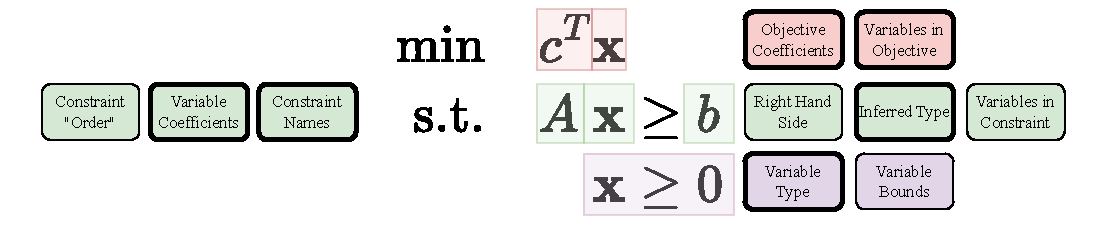
\includegraphics[scale=0.8]{Bilder/DrawIO/model_information}
			\caption{All parts of a model that contain useful information for semantic grouping of constraints and variables. Elements with a thick border are already used as a key concept in one of the existing detectors.}
			\label{fig:tree:information}
		\end{figure}

		Before we present any algorithmic details, we give an overview about the available information which might be used to define suitable strategies. \todo{roter Faden}

		\begin{enumerate}
			\item \textbf{Objective}: For the objective functions, information about the participating variables and their coefficients is available. For some models e.g. for Bin-Packing, this information alone is sufficient to partition the variables.
			\item \textbf{Coefficients}:
			The use of coefficients to classify constraints and variables was already in discussed in Section \ref{chap:gcg:classifiers}.
			\item \textbf{Bounds}: For all variables $lb \leq x \leq ub$ information about their lower- and upper-bounds is available.
			Furthermore, the left- and right-hand-side of linear constraints $lhs \leq \sum_i a_i x_i \leq rhs$ are available as well.
			\item \textbf{Types}: Variable types such as \textit{Integer} are usually stated explicitly in the input format. If not, then information about the variable bounds can be used to deduce a type, e.g. $0 \leq x \leq 1$ is a strong indicator that $x$ is a \textit{Binary} variable.
			\item \textbf{Names}: If specified by the modeler, then variables and constraints might have meaningful names which can be used as a strong indicator which constraints and variables belong to the same group.
			\item \textbf{Order}: In contrast to other kinds of information, the constraint \enquote{order} is no intrinsic property of the model itself. With the term \enquote{order}, we refer to the order of the constraints as specified in the input format. When a model is created e.g. via. a script, constraints are usually added in \textit{blocks} by the modeler. This information is used in Section \ref{chap:tree:classifiers:voting} to conceptualize a classifier based on that.
		\end{enumerate}

	\section{Classifiers}
	\label{chap:tree:classifiers}
	% 2 Seite

		In the following Sections we describe different classifiers which are not yet implemented in \ac{GCG} but could potentially provide new information about the model.
		Adding new classifiers has, in addition to practical implications such as higher maintenance overhead, additional side-effects regarding runtime and memory requirements.
		Each new classifier provides new opportunities for existing detectors to find new partial decompositions.
		This can prove especially useful for detectors like consclass, which directly depend on the found classifications.
		On the other hand, this dependence can result in a sub-optimal runtime investment if the found classifications provide no new information, because the generated partial decompositions based on that will most certainly be of bad quality as well. \todo{wording}
		Therefore, we will refrain from mentioning all missing model properties for which a classifier \textit{could} be built, and only focus on promising candidates.
		\todo{Summarize goals for custom classifiers}

		\subsection{Bounds}

			When considering bounds, we differentiate between variables and constraint respectively.

			\subsubsection{Variable bounds}

				The classifier for variable bounds can be considered as a simple mapping from pairs of bounds to a unique class index.
				More formally, given a list of all unique pairs of lower and upper bounds for variables $B = (b_1, b_2, \ldots, b_k)$, with $b_i \in \mathbb{Q} \times \mathbb{Q}$, we map each variable to the index of its bounds in $B$.
				This mapping is trivially unique.

				Mapping the variables in the described way has the side-effect that $0 \leq x \leq 1$ and $y \in \{ 0, 1 \} $ are mapped to the same class.
				This behavior is able to account for missing declarations of variables as binary in the input format read by \ac{GCG}.
				The classification is wrong if $x$ is truly meant to be a continuous variable, but this is offset by the fact that \ac{GCG} already includes a classifiers based on \ac{SCIP} types, which will correctly classify both variables in this case.

				Types of models where information about the variable bounds \textit{can} be leveraged include instances of e.g. Container Loading.
				Here, variables $x, y, z \in \mathbb{R}$ encoding the positions of parcels to be loaded into a container are continuous. If the container is not a cube, i.e., it has a different length in each spacial dimension, then the variables have to have different bounds.

			\subsubsection{Constraint bounds}

				A classifier for constraint bounds works in a similar manner as for variables.
				By collecting all bounds and assigning a class to each constraint based on that list, we obtain a unique mapping.
				Note that for inequalities the absolute value either of the two bounds will always be infinity. For equalities which were not replaced with equivalent inequalities, both bounds will be equal.

				In addition to a classifier based on the actual \textit{values} of the bounds, i.e., for values $a, b \in \mathbb{R}$ of a linear constraint $a \leq \sum a_i x_i \leq b$, we propose a classifier based on the \textit{sign} of  $a$ and $b$.
				Here, the linear constraint is transformed to standard form to prevent a different classification for equivalent constraints in case the constraint is multiplied by $-1$.
				Therefore, only four potential classes shown in Table \ref{table:tree:classifiers:bounds:exist} remain.
				This classifier can be used for variables analogously.

				\begin{table}[ht!]
					\centering
					\begin{tabular}{l|l|l|l}
						\textbf{Class Nr.} & \textbf{Name} & \textbf{$sign(a)$} & \textbf{$sign(b)$} \\
						\toprule
						\toprule
						1 & Positive & $+$ & $+$ \\
						2 & Mixed &$+$ & $-$ \\
						2 & Mixed & $-$ & $+$ \\
						3 & Negative & $-$ & $-$ \\
						4 & Zero $(a = b = 0)$ & $+/-$ & $+/-$
					\end{tabular}
					 \caption{The four classes of the sign-variant of the bounds classifier.}
					 \label{table:tree:classifiers:bounds:exist}
				\end{table}

				\todo{cap. lot sizing example}

				\clearpage

		\subsection{Relaxed MIPLIB types}

				\begin{table}[ht!]
				\centering
				\begin{tabular}{l|l|l|l}
					\textbf{Nr.} & \textbf{Type} & \textbf{Linear Constraint} & \textbf{Notes} \\
					\hline
					\hline
					1 & Empty & $\emptyset$ & - \\
					2 & Free & $-\infty \leq x \leq \infty$ & No finite side. \\
					3 & Singleton & $a \leq x \leq b$ & - \\
					4 & Aggregation & $ax + by = c$ & - \\
					5 & Precedence & $ax - ay \leq b$ & $x$, $y$ have same type. \\
					6 & Variable Bound & $ax + by \leq c$ & $x \in \{0, 1\}$ \\
					7 & Set Partitioning & $\sum 1 x_i = 1$ & $\forall i: x_i \in \{0, 1\}$ \\
					8 & Set Packing & $\sum 1 x_i \leq 1$ & $\forall i: x_i \in \{0, 1\}$ \\
					9 & Set Covering & $\sum 1 x_i \geq 1$ & $\forall i: x_i \in \{0, 1\}$ \\
					10 & Cardinality & $\sum 1 x_i = b$ & $\forall i: x_i \in \{0, 1\}, b \in \mathbb{N}_{\geq 2}$ \\
					11 & Invariant Knapsack & $\sum 1 x_i \leq b$ & $\forall i: x_i \in \{0, 1\}, b \in \mathbb{N}_{\geq 2}$ \\
					12 & Equation Knapsack & $\sum a_i x_i = 1$ & $\forall i: x_i \in \{0, 1\}, b \in \mathbb{N}_{\geq 2}$ \\
					13 & Bin Packing & $\sum a_i x_i + ay \leq a$ & $\forall i: x_i, y \in \{0, 1\}, b \in \mathbb{N}_{\geq 2}$ \\
					14 & Knapsack & $\sum a_i x_i \leq b$ & $\forall i: x_i \in \{0, 1\}, b \in \mathbb{N}_{\geq 2}$ \\
					15 & Integer Knapsack & $\sum a_i x_i \leq b$ & $\forall i: x_i \in \mathbb{Z}, b \in \mathbb{N}$ \\
					16 & Mixed Binary & $\sum a_i x_i + \sum p_j s_j \; \{\leq, =\} \; b$ & $\forall i: x_i \in \{0, 1\}, \forall j: s_j \; \mathrm{continuous}$ \\
					17 & General Linear & $\sum a_i x_i \; \{\leq, \geq, =\} \; b$ & No special structure.
				\end{tabular}
				\caption{The structure of all constraint types which the \textit{relaxed} version of the MIPLIB classifier detects.}
				\label{table:constypes:relaxed}
			\end{table}

			In order to mitigate \textit{some} of the issues

			Similar to the MIPLIB classifier, all types can be deduced from local information only. Thus, one pass over the constraint matrix is sufficient to classify all constraints according to Table \ref{table:constypes:relaxed}. \todo{WIP}

			\clearpage

		\subsection{Voting}
		\label{chap:tree:classifiers:voting}

			As mentioned earlier, the motivating idea behind each individual classifier is to group constraints according to some property, while the type of this property can vary greatly between classifiers.
			Under the assumptions that groups of constraints share at least \textit{some} of these properties and are thus assigned to the same classes, we can define a new type of classifier.
			Note that this classifier can be equivalently conceptualized as an additional \textit{strategy}, which are the basic building blocks of the refinement algorithm and explained in Section \ref{chap:tree:strategies}.
			This assumption is, at least on examples that can be observed in practice, a reasonable one.

			\subsubsection{Voting (unordered)}

				\begin{figure}[ht!]
					\centering
					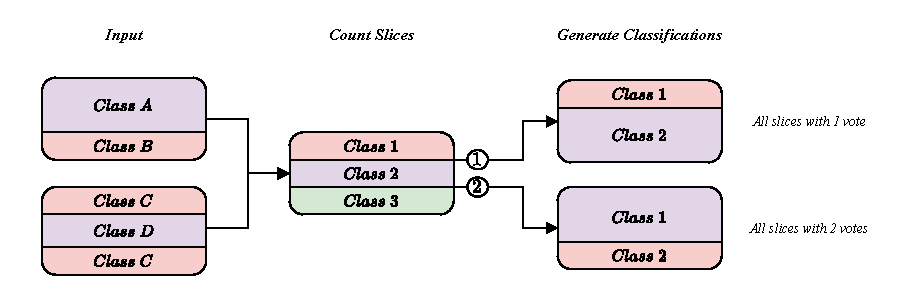
\includegraphics[scale=1.05]{Bilder/DrawIO/strat_ordered_voting_pdf}
					\caption{text}
					\label{fig:tree:classifiers:ovoting}
				\end{figure}

				In order to derive a simple and efficient algorithmic approach to this problem, we can make an additional assumptions not based on the model itself, but on its representation in common input formats like \lstinline|.lp| and \lstinline|.mps| files.
				A lot of models are generated via. scripts and written to such files for portability and interoperability with other solvers.
				One exploitable property which can be observed in a lot of models is, that groups constraints are usually \textit{added in bulk}.
				This results in consecutive blocks of constraints which are semantically related, which is illustrated in the \enquote{Input} column of Figure \ref{fig:tree:classifiers:ovoting}.
				If a class of constraints is split into two non-consecutive groups like the second partition from Figure \ref{fig:tree:classifiers:ovoting}, then we can deduce that they are meant to be two different groups.

			\subsubsection{Voting (unordered)}
			\label{chap:tree:classifiers:cooccurence}

				If the read model does \textit{not} have the property of properly ordered constraint blocks, a more involved algorithmic approach can be used.
				Here, the general problem can be reduced to group constraints with each other which are \textit{often} assigned to the same class.
				Given a set of partitions $Q = \{ \pi_1, \pi_2, \ldots, \pi_k \}$, we can compute a matrix  $A = (n_{ij})_{1 \leq i, j \leq m}$ which contains the pair-wise occurrences of all elements with $m$ being the number of constraints in total.
				Here, the set of partitions $Q$ might correspond to the found classifications in e.g. \ac{GCG}s classification stage.
				Each entry $n_{ij}$ can be computed by using Equation \ref{eq:tree:classifiers:cooccurence}.
				%
				\begin{equation}
				\label{eq:tree:classifiers:cooccurence}
					n_{ij} = | \{ x \mid \forall \pi \in Q, i \in \pi, \forall x \in \pi \} |
				\end{equation}
				%
				If all entries are computed the matrix requires $O(m^2)$ space in memory, which is not feasible for large models. A simple method to reduce the memory requirements of $A$ is the concept of a \textit{sparse matrix}, i.e., only those $n_{ij} \neq 0$ are actually held in memory.

				For set of partitions in which the individual cells do not \enquote{agree} with each other, i.e., it holds that $n_{ij} \geq 0$ for almost all pairs, we propose a heuristically approach based on min-heaps.
				A min-heap is a tree-like data-structure always maintaining the invariant that the key associated with a node $P$ is less than or equal to the keys associated with all nodes that are children of $P$.
				We associate one min-heap with each constraint of maximum size $a \leq m$.

				\begin{algorithm}[ht!]
					\centering
					\begin{algorithmic}
						\Require Set of partitions $Q = \{ \pi_1, \pi_2, \ldots, \pi_k \}$
						\Statex
						\Function{VotingUnordered}{Q}
							\State $heaps \gets m$ min-heaps
							\For{$\pi \in Q$}
								\For{$x, y \in \pi$}
									\State \Call{PushPair}{heaps[x], }
								\EndFor
							\EndFor
						\EndFunction
					\end{algorithmic}
					\caption{a}
					\label{algo:tree:classifiers:cooccurence}
				\end{algorithm}

				An additional pre-processing step can be done by e.g. filtering out cells of partitions whose entropy is below a certain threshold or not removing trivial partitions before computing $A$.

				\clearpage

%	\section{Tree Refinement}
%	% 4 Seiten
%
%		\begin{figure}[ht!]
%			\centering
%			\includesvg{Bilder/Hierarchy/hierarchy_binpack_NOP}
%			\caption{Test}
%			\label{fig:tree:binpackNOP}
%		\end{figure}

	\section{Strategies}
	\label{chap:tree:strategies}

		Strategies are \textit{the} central building block of the algorithm and are responsible for refining sets of constraints or variables.
		Let $U$ be a the total set of constraints or variables.
		Each strategy can be formalized as a function $f: S \rightarrow \Pi(S)$ which gets a single set $S \subseteq U$ as input and produces a partition $\pi \in \Pi(S)$ as output.
		Conceptually, each strategy can be seen as a materialization of a specific splitter function as defined in Section \ref{chap:prelims:partitionref}.

		%In the following, we differentiate between re-callable and non re-callable strategies. The former type may be called more than once in any given sub-tree, as the result may depend on precise position of the node that is being expanded.

		\subsection{Slice (Partition)}
		\label{chap:tree:strategies:slice:part}

			\begin{figure}[ht!]
				\centering
				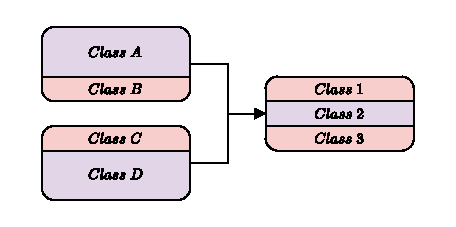
\includegraphics[scale=1.2]{Bilder/DrawIO/strat_slicing_pdf}
				\caption{A simplified illustration assuming that constraint in both partitions can be rearranged into continuous blocks, thus \enquote{slicing} the partitions into different-sized chunks. The output partition inherits all these slices.}
				\label{fig:tree:strat:slice}
			\end{figure}

			Slicing strategies are the most simple type of strategy.
			Given two partition $\pi, \pi' \in \Pi(U)$, we define the \textit{combined partition} $\pi \sqcap \pi'$ as follows:
			%
			\begin{equation}
				\label{eq:tree:strat:slice:overlay}
				\pi \sqcap \pi' = \{ A_i \cap B_j \mid A_i \in \pi, B_j \in \pi' \} \setminus \emptyset
			\end{equation}
			%
			This concept is illustrated in Figure \ref{fig:tree:strat:slice}.
			Because strategies only refine single sets and not whole partitions, Equation \ref{eq:tree:strat:slice:overlay} always degenerates to $\pi_{slice} \sqcap \{ S, U \setminus S \}$ for some partition $\pi_{slice} \in \Pi(U)$ and a set $S$ we want to refine.
			The result is then restricted to elements of $S$, which yields a partition of $S$.
			More formally, this strategy can be expressed as Function \ref{eq:tree:strat:slice:function} and computed efficiently using Algorithm \ref{algo:tree:strat:slice}.
			%
			\begin{equation}
			\label{eq:tree:strat:slice:function}
				f_{\pi_{splitter}}(S) = \left\{ A_i \cap S \mid A_i \in \pi_{splitter} \right\} \setminus \emptyset
			\end{equation}
			%
			Note that the operator $\sqcap$ is trivially associative, i.e., $(\pi \sqcap \pi') \sqcap \pi'' = \pi \sqcap (\pi' \sqcap \pi'')$:
			%
			\begin{alignat*}{4}
				X \in (\pi \sqcap \pi') \sqcap \pi'' &\iff \exists Z \in (\pi \sqcap \pi'), C \in \pi'' && : \; && X && ={} Z \cap C \\
				&\iff \exists A \in \pi, B \in \pi', C \in \pi''&& : \; && X && ={} (A \cap B) \cap C \\
				&\iff \exists A \in \pi, B \in \pi', C \in \pi''&& : \; && X && ={} A \cap (B \cap C) \\
				&\iff  X \in \pi \sqcap (\pi' \sqcap \pi'')
			\end{alignat*}

			In conjunction with commutativity, this fact can be used to e.g. eliminate part of the search space by pruning duplicated nodes in the tree and only expanding one instance of any given sub-tree.

			A simple example where two successive applications of this slicing strategy can

			\begin{algorithm}[ht!]
				\centering
				\begin{algorithmic}
					\Require Partition $\pi = \{ A_1, A_2, \ldots, A_k \}$, set $S \subseteq U$, function $f_C: U \mapsto \mathbb{N}$ for $C = \{ C_1, C_2, \ldots \} \in \Pi(U)$ mapping $u \in U$ to $C_i$ iff $u \in C_i$
					\Ensure Partition of $S$ according to Function \ref{eq:tree:strat:slice:function}.
					\Statex
					%
					\Function{strategySlice}{$\pi, S$}
						\State $\pi_{out} \gets$ list of $k$ empty sets $B_1, B_2, \ldots, B_k$
						\For{$s \in S$}
							\State $i \gets f_S(s)$
							\State $B_i \gets B_i \cup \{ s \}$
						\EndFor
						\State Remove empty sets from $\pi_{out}$
						\State \Return $\pi_{out}$
					\EndFunction
				\end{algorithmic}
				\caption{If a lookup table represented by function $f$ is available, then Function \ref{eq:tree:strat:slice:function} can be implemented in O($|S|$).}
				\label{algo:tree:strat:slice}
			\end{algorithm}

			\FloatBarrier
			\clearpage

		\subsection{Slice (Covering)}

			\begin{figure}[ht!]
				\centering
				\includesvg[scale=1.25]{Bilder/DrawIO/setcov}
				\caption{Given $U = \{ 1, \ldots, 6 \}$, and $S = \{ \{ 1, 2, 3 \}, \{ 3, 4 \}, \{ 4, 5, 6 \} \} \subseteq 2^U$, with each $C \in S$ corresponding to one \textit{feature}.
				Each element $x \in U$ is part of at least one set $C \in S$, thus possessing at least one feature.
				This example can be encoded as a graph, where the right side \enquote{the features} are pre-partitioned into individual cells. By applying the standard partition refinement framework from Section \ref{chap:prelims:partitionref} with function \ref{eq:prelims:pref:exists}, we obtain a partition $\pi \in \Pi(U)$ in which the elements any given cell possess the same features.}
				\label{fig:tree:strat:cov}
			\end{figure}

			%Before we explain the \textit{covering} version of the previous strategy, Function \ref{eq:tree:strat:slice:function} can be seen as an instantiation f
			Let $U$ be an arbitrary set. Then a covering can be defined as a set $S \subseteq 2^U$, where $S^U$ denotes the power set, such that:
			%
			\begin{equation*}
				U = \bigcup_{C \in S} C
			\end{equation*}
			%
			The definition is equivalent to a set partitioning without the condition that sets of $S$ must be pairwise disjuct.
			Each set $C \in S$ corresponds to one \textit{feature}, with the elements $x \in C$ considered to possessing said feature.
			The goal of the covering version of the slicing strategy is to partition the elements of a given set in such a way, that elements in the same cells all possess the same features.
			In order to obtain such a partition from a set covering $S$, we can encode the underlying problem as a graph and use the standard partition refinement framework.
			%The splitter-function that is being used here corresponds to Function \ref{eq:prelims:pref:exists}.
			Afterwards, the resulting partition can be used to slice the given set as described in Section \ref{chap:tree:strategies:slice:part}.

			The strategy can be used to e.g. partition constraints according to the types of variables that they contain.
			It is functionally equivalent to the refinement method \enquote{fast} from \cite{salvagninDetectingSemanticGroups2016}.
			The name most likely stems from an algorithm informally described a fast algorithm based on bucket sort to implement such a partition refinement algorithm. \todo{Example}

			\clearpage

		\subsection{Recursive}

			\begin{figure}[ht!]
				\centering
				\includesvg[scale=1.25]{Bilder/DrawIO/strat_rec}
				\caption{An example of a graph for which the partition refinement algorithm takes multiple iterations to yield a stable partition (Function \ref{eq:prelims:pref:exists}). Red circles around the vertices highlight changes to the cells in the respective iterations. The algorithm is initialized with $\pi_{init} = \{ \{ 1, 2 \}, \{ 3, 4 \}, \{ A, B, C, D \} \}$. During the first iteration, all vertices on the right side are in the same cell so no changes can happen on the left side. Vertices $A, B$ are not connected to cell $\{ 3, 4 \}$. A similar reasoning applies for the second iteration.}
				\label{fig:tree:strat:rec}
			\end{figure}

			The \textit{recursive} strategy is the the only strategy which needs to utilizes the full blown partition refinement framework.
			The strategy is based on the canonical constraint-variable un-directed graph already shown in Figure \ref{fig:prelims:graphs:binpackbipartite}.
			Each variable and constraint corresponds to exactly one vertex, while an edge between a constraint and variable node exists iff the variable is part of the constraint.
			More formally, given a set of constraints $C = \{ c_1, \ldots, c_m \}$ and a set of variables $X = \{ x_1, \ldots, x_n \}$. Let $a_{ij}$ be the coefficient of variable $x_i \in X$ in constraint $c_j \in C$.
			Then we can define the graph as follows:
			%
			\begin{equation*}
				G = (V, E) = (X \cup C, \{ \{ x_i, c_j \} \mid x_i \in X, c_j \in C, a_{ij} \neq 0 \})
			\end{equation*}
			%
			The size of the graph in terms of it's edges and vertices depends entirely to the underlying problem.
			A partition is obtained by running the algorithm with either Function \ref{eq:prelims:pref:count} or Function \ref{eq:prelims:pref:exists}.
			Afterwards, the partition is used to slice a given set according to the method described in Section \ref{chap:tree:strategies:slice:part}.
			Note that even thought the generated graph is always bi-partite, it does not necessarily fulfill the conditions mentioned in Section \ref{chap:prelims:partitionref} for the fast variant of the refinement algorithm, i.e., that all nodes on one of the two sides of the bi-partite graph are all in their own cell.
			As a consequence, one full execution of the recursive strategy might take orders of magnitude longer than an execution of one of the two slice variants explained previously. \todo{"orders of magnitude" ein wenig übertrieben}

			\clearpage

	\section{Cutoff Conditions}
	\label{chap:impl:cutoff}

		In order to limit the size of the tree and ensure that we only explore relevant parts of the search space, we propose several conditions the terminate the search early on.
		The conditions can be divided into two groups:

		\begin{enumerate}
			\item \textit{Local} Conditions, which can be evaluated by only considering information about one \textit{singular} node or its immediate predecessor.
			\item \textit{Global} Conditions, whose evaluation requires information about e.g. the precise path to the node, i.e., its position in the tree and therefore information about its ancestors, \textit{or} requires knowledge about other nodes or completely distinct sub-trees.
		\end{enumerate}

		Note that the following conditions are only \textit{correct} for the strategies presented in Section \ref{chap:tree:strategies}, which are all a specialized version of the partition slicing strategy.
		In the following, let $T = \srt$ be a \ac{SRT}.

		\subsection{Local Conditions}
		% 1 Seite

			With access only to local information, these conditions are restricted to the information about a single node $v_0 \in V$.

			\subsubsection{Refined Partition Size}

			Assuming a proper ground-truth is available or any heuristic information about the potential size $k \in \mathbb{N}$ of the target partition, many found nodes can be excluded from the scoring a-priori. \todo{WIP}
			We can terminate the search for any sub-tree rooted at $v_0$ if $| \mathrm{Cells}_{v_0} | \gg k$.
			Here, the motivation is that in any partition $\pi$ computed in the post-processing in which $v_0$ is participating, $|\pi| \gg k$ holds.

			\subsubsection{No Changes}

			As soon as the algorithm expands a set $S$ with a strategy, we get a partition $\pi \in \Pi(S)$ as a result.
			If $S \in \pi$, this implies that $\pi = \{ S \}$ and the strategy did not refine $S$ any further and we can terminate the search for the current sub-tree.

		\subsection{Global Conditions}
			% 1 Seite

			As mentioned before, global conditions are more flexible and allow for more involved logic to be executed.

			\subsubsection{Sub-Tree Duplication}

				\begin{figure}[ht!]
					\centering
					\includesvg[scale=0.7]{Bilder/DrawIO/subtree_virtual_ref}
					\caption{Node B is a duplicate of Node E, but the latter was added to the tree before Node B. Thus, as soon as Node B is created this duplication is detected and is never added to the tree. Because this is just an optimization to improve runtime, we have to act \textit{as if} Node B was expanded. Thus, a dummy node is created which \textit{refers} to Node E to keep e.g. the scoring system functional.}
					\label{fig:tree:cutoff:subtree}
				\end{figure}

				If $v_0$ is expanded by the algorithm, then all cells of the node are expanded in the same way by all strategies that did not run previously.
				The expansion of a cell by a certain strategy usually results in a new tree node, which is in turn expanded during a future iteration of the algorithm.
				If a new node that is about to be added already exists somewhere else in the tree, i.e., there is a already an equivalent tree node present, the expansion can stop at that point, since it would lead to the same subtree structure and therefore redundant computation.
				Here, two tree nodes are considered \enquote{equivalent} if they consist of the same cells, i.e., $v_i = v_j \iff \mathrm{Cells}_{v_i} = \mathrm{Cells}_{v_j}$. An example of this condition is illustrated in Figure \ref{fig:tree:cutoff:subtree}.

			\subsubsection{Most Optimistic Partition Size}

				Similar to the local condition terminating the search at a node $v \in V$ exceeding a certain number $k \in \mathbb{N}$ of cells, we can terminate the search as it becomes evident that the size of \textit{any} partition containing $v$ and is generated by function \ref{eq:tree:scoring:partcomp} will exceed $k$.
				This \textit{Most optimistic partition size}, i.e., the size of the smallest partition that can be generated using $v$, can be computed as shown in Function \ref{eq:tree:cutoff:mos}.
				%
				\begin{equation}
				\label{eq:tree:cutoff:mos}
					\mathrm{MOS}(v) = \begin{cases}
						0 & \text{if} \; v = R \\
						|\mathrm{Cells}_{\mathrm{ParentNode}_v}| + \mathrm{MOS}(\mathrm{ParentNode}_v) - 1 & \mathrm{otherwise}
					\end{cases}
				\end{equation}
				%
				Because all nodes in the \ac{SRT} are non-empty, it trivially holds that $\mathrm{MOS}(v) \geq \mathrm{MOS}(\mathrm{ParentNode}_v)$ for all $v \in V$.
				As soon as $MOS(v) \gg k$, we can terminate the search as all partitions generated using at last one descendant of $v$ will exceed the threshold.

		\subsubsection{Depth}

			Under the assumption that most of the \enquote{interesting} sets are found early, it could be beneficial to abort the search for a sub-tree as soon as a certain depth has been reached.
			The depth of a certain node $v \in V$ can be computed using a simple recursion to the root node:

			\begin{equation*}
				\mathrm{Depth}(v) = \begin{cases}
					0 & \text{if} \; v = R \\
					1 + \mathrm{Depth}(\mathrm{ParentNode}_v) & \mathrm{otherwise}
				\end{cases}
			\end{equation*}

			This condition should be used with care, as more complex models will most likely require multiple iterations of the algorithm until the \ac{SRT} has been enriched with enough information to reverse-engineer the original formulation.

			\clearpage

		\subsubsection{Side effects of global conditions}

			\begin{figure}[ht!]
				\centering
				\begin{minipage}[t]{0.45\textwidth}
					\vspace{0pt}
					\includesvg[scale=0.65, inkscapelatex=false]{Bilder/DrawIO/side_effects_left}
					\caption{a}
					\label{fig:tree:cutoff:sideeffect:a}
				\end{minipage}
				%
				\begin{minipage}[t]{0.45\textwidth}
					\vspace{0pt}
					\includesvg[scale=0.65, inkscapelatex=false]{Bilder/DrawIO/side_effects_right}
					\vfill
					\caption{a}
					\label{fig:tree:cutoff:sideeffect:b}
				\end{minipage}
				\caption{text}
				\label{fig:tree:cutoff:mos}
			\end{figure}
			\todo{Falsches Bild}

			Conditions such as \textit{Depth} or \textit{Most Optimistic Partition Size} can have unintended side-effects in combination with other global conditions like \textit{Sub-Tree Duplication}.
			As shown in Figures \ref{fig:tree:cutoff:sideeffect:a} and \ref{fig:tree:cutoff:sideeffect:b} with identical Nodes B and D, the \ac{SRT} can have a different structure depending on the \textit{order} of node expansion. In the visualizations, nodes were expanded in the order of numbers shown in small circles attached to the nodes. During expansion, the only active cutoff-cconditions were the aforementioned \textit{Sub-Tree Duplication} and \textit{Depth}, which cut off all nodes below or at a depth of 3.

			In Figure \ref{fig:tree:cutoff:sideeffect:a}, Node B was added to the tree before Node D, thus cutting off the tree after the latter.
			The sub-tree rooted at Node B was expanded further, until the \textit{Depth}-condition became active.
			In Figure \ref{fig:tree:cutoff:sideeffect:b}, the exact opposite happened. Node D was expanded before Node B, which resulted in the creation of Node C before a sufficient cutoff depth has been reached.

			In the case of \textit{Sub-Tree Duplication} and \textit{Depth}, expanding the tree in breath-first order solves the described problem, but side-effects with other conditions are still possible. Thus, depending on the precise set of implemented conditions, one has to evaluate possible side-effects.

	\clearpage

	\section{Scoring}
	\label{chap:gcg:scoring}
	% 1 Seite

		Up until this point we have only described how the algorithm refines sets based on different strategies, despite the goal being a list of promising partitions.
		Before we describe how to select such partitions, we have to define how we actually \textit{get} a list of partitions from the refinement tree.

		Let $G = (V, R, E)$ the set refinement tree with vertex set $V$, designated root node $R \in V$ and edges $E \subseteq V \times V$. \\
		Let $Recombine_k(U_1, U_2, \ldots, U_k): U_1 \times U_2 \times \ldots \times U_k \xrightarrow{} 2^{U_1 \cup U_2 \cup \ldots \cup U_k}, k \in \mathbb{N}$ be a Function defined as follows:
		%
		\begin{equation*}
			Recombine_k(U_1, U_2, \ldots, U_k) = \begin{cases}
				\emptyset & k = 0 \\
				U_1 & k = 1 \\
				\{ \{ u \} \cup r \mid u \in U_1, r \in Recombine_{k-1}(U_2, U_3, \ldots, U_k) \} & else
			\end{cases}
		\end{equation*}
		%
		More informally, $Reombine_k$ takes a total of $k$ arbitrary sets $U_1, \ldots, U_k$ and computes a set containing all possible $k$-tuples $(u_1, u_2, \ldots, u_k)$ with $u_i$ restricted to elements from $U_i$.
		Thus, the set of \textit{all} partitions constructible from a sub-tree rooted at vertex $v \in V$ can be computed using Function \ref{eq:tree:scoring:partcomp}.
		%
		\begin{equation}
		\label{eq:tree:scoring:partcomp}
			Partitions(v) = \begin{cases}
				Sets(v) & \text{if $v$ is leaf node} \\
				\left\{ Recombine_{|Sets(v)|} \right\} & else
			\end{cases}
		\end{equation}
		\todo{WIP}
		%
		It is clear that setting $v = R$ gives the set of all possible partitions.
		\todo{Add simple proof}

		One can deduce from the definition of Function \ref{eq:tree:scoring:partcomp} that the number of partitions depends on the depth and maximum out-degree of any given node of the tree.
		Therefore, it will be of vital interest to only consider \enquote{interesting} sets.
		Ideas and possible implementations are discusses in Chapter \ref{chap:impl}.

		\clearpage

		\subsubsection{Example}

			\begin{figure}[ht!]
				\centering
				\includesvg[scale=0.5, inkscapelatex=false]{Bilder/Hierarchy/scoring_example}
				\caption{A sample \ac{SRT} with four nodes. Node 1 has one descendant, so the recursive function will generate multiple possible partitions because of that.}
				\label{fig:tree:scoring:example}
			\end{figure}

			In order to illustrate the generation of partition from a given \ac{SRT}, we use the tree shown in Figure \ref{fig:tree:scoring:example} as an example.
			In the following, we abbreviate a node \enquote{Node $i$} with $N_i$.
			Applying the definition of Function \ref{eq:tree:scoring:partcomp} to the \ac{SRT}, we have start at the root node with identifier 0.
			%
			\begin{equation*}
				Partitions(N_0) = {Recombine}_1
			\end{equation*}
			\todo{WIP}
			%
			Because the root node only consists of one cell, we just take the union of $Partitions(N_1)$ and $Partitions(N_3)$.
			For the latter, we can compute the result easily, because $N_3$ is a leaf node. Thus, the set of all possible ways of generating partitions for cell 0 in this sub-tree consists of the single partition $\{ \{ 1, 3, 4 \} \}$
			For $N_1$, we have to execute the recursion twice:

			\begin{enumerate}
				\item The first possibility to partition cell 0 is $\{ 1, 2 \}$.
				\item In addition, we have another option to partition set $2$: $\{ 3, 4 \}$, which is possible because of Node 9.
			\end{enumerate}

			Thus, we can partition cell 0 in this sub-tree in two ways: $\{ \{ 1, 2 \}, \{ 1, 3, 4 \} \}$.
			The union of the left and right sub-tree results in three possible ways to partition cell 0, finishing the partition generation phase.

		\clearpage

		\subsection{Constraint Names}
		\label{chap:tree:scoring:names}

			One important piece of information that usually reflects the modelers \textit{intent} when it comes to the semantic difference are the names of the constraints or variables, in the following abbreviated with just \enquote{names}.
			As discusses in Section \ref{chap:gcg:classifiers:name}, names usually consist of multiple parts, with one part containing all the information related to \textit{semantics}.
			Extracting this part of the name can be done heuristically using Algorithm \ref{algo:tree:scoring:nameheur}.
			The heuristic consist of four major steps:
			\begin{enumerate}
				\item Remove \textit{modifies} which are usually enclosed in either brackets or some other special character combination which consists of an \textit{opening} and \textit{closing} character.
				\item \enquote{Normalize} the string by replacing any non-alpha-numeric separators such as spaces, tabs, $\ldots$ with a single character $c$ such as \enquote{\_}.
				\item Split the string according to $c$ and try to detect the part with the relevant semantics.
				\item \textit{(Optional)} Remove any left-over non-alpha characters such as numbers.
			\end{enumerate}

			Step 4 is explicitly marked as optional, because sometimes numbers are integral part of the name, sometimes they are not.
			Both of these cases can actually be observed in the same model \footnote{StrIPlib UUID: d48c9568-e0ea-4c77-9a3b-b7f4dc530d5f}.
			For this model in particular, the constraints \enquote{cut1} to \enquote{cut4} are of interest.
			The constraints with the prefix \enquote{cut1} and \enquote{cut2} are structurally identical, i.e, the they all share the same number of non-zeros and the same type of variables, while \enquote{cut3} and \enquote{cut4} do not.
			Here, \enquote{cut1} and \enquote{cut2} would have to belong to the same group, while \enquote{cut3} and \enquote{cut4} belong in a group their own.
			With the heuristic as is, this case is not detected with or without step 4 because additional information about the actual structure of constraint is required.

			Note that the Algorithm makes some implicit key assumptions, such as:
			\begin{itemize}
				\item That the name actually carriers any semantically relevant information at all.
				\item The names adhere to a \enquote{common} format, i.e., the modifier comes \textit{after} the semantics part. Here, constraint names such as \enquote{capacity\_bin\_k}, \enquote{out\_flow\_k} qualify, but the same names in reverse do not.
			\end{itemize}

			These assumptions proved reasonable for almost all models observed in practice which had proper names available. Still, there cases where this approach fails \todo{Give MIPLIB examples}.

			\begin{algorithm}[ht!]
				\centering
				\begin{algorithmic}
					\Require Name of a constraint
					\Ensure Relevant semantics of the constraint name if the name adheres
					\Statex
					%
					\Function{extractSemanticPart}{$name$}
						\State ${name}_{new} \gets name$
						\State ${name}_{old} \gets name$
						\Repeat
							\State ${name}_{old} \gets name$
							\State $start \gets$ Position of opening character e.g. $\lbrack$, \{, (, $\ldots$
							\State $end \gets$ Position of corresponding closing character e.g. $\rbrack$, \}, ), $\ldots$
							\State ${name}_{new} \gets {name}_{old}$ without characters in range $[start, end]$
						\Until{${name}_{new} = {name}_{old}$}
					\EndFunction
				\end{algorithmic}
				\caption{}
				\label{algo:tree:scoring:nameheur}
			\end{algorithm}
			\todo{WIP}

			As soon as the semantic part of all names is extracted, constraints and variables can be grouped based on this information.
			Possible post-processing steps might include an application of the mentioned Levenshtein-Distance from Chapter \ref{chap:gcg}.
			Even thought the Algorithm has quadratic time complexity and is therefore unlikely to be used with the full set of original constraint or variable names, a reasonable assumption is that
			%
			\begin{equation*}
				\{ \; \Call{ExtractSemanticPart}{Name(c)} \mid c \in Cons \; \} \ll \{ \; Name(c) \mid c \in Cons \; \}
			\end{equation*}
			%
			Analogously, the assumption is made for variable names as well.
			Thus, an Algorithm for the Levenshtein-Distance, even under worst-case considerations, might be applicable and thus resulting in a better partitioning.

			\clearpage


		\subsection{Ground Truth based}
		\label{chap:tree:scoring:groundtruth}
		% 1 Seite

			As discusses in the previous Sections, the algorithm starts with a set in which all constraints or variables are in the same cell.
			In order to \textit{guide} the search towards a plausible semantic partitioning, the existence of a ground-truth partition which approximates the desired partition reasonably well can be used to terminate the search or select promising partitions after the search-space has been explored.
			Terminating the search can, in practice, be very useful, because preventing the algorithm from expanding a node not only prevents unnecessary work being done for this particular node, but also prevents the generation of the entire sub-tree below; reducing the number of potential candidate partitions and overall runtime and space requirements of the algorithm.

			Potential sources for a suitable ground-truth partitions include
			\begin{itemize}
				\item Constraint names using the heuristic from Section \ref{chap:tree:scoring:names}.
				\item Variable information, i.e., given a ground-truth of semantic groupings of variables, one could obtain a corresponding ground-truth partition for constraints by assigning two constraints to different groups iff they contain different kinds of variables according to the ground-truth.
			\end{itemize}

			Without the availability of a reasonably ground-truth, it is currently unclear how to know when to terminate the search and more importantly, what structured the desired target partitions should have.
			Here, the term \enquote{structure} refers to all relevant properties of the target partition, including but not limited to, the number and size of the cells.

			Assuming a reasonable ground-truth has been obtained, a partition-comparing score such as the Rand-Index already discussed in Section \ref{chap:prelims:rand} can be used a number of promising candidates.
			Furthermore, the refinement can be terminates for sets which are already \textit{homogeneous} according to the ground-truth partition.
			The idea being is that by refining the set further we do not gain any new information.
			\todo{completeness missing}

			\clearpage

		\subsection{Connected Components Score}
		% 1 Seite

			The ground-truth based scoring from Section \ref{chap:tree:scoring:groundtruth} scores candidates based on a partition $\pi$, which is assumed to resemble a semantic grouping reasonable close to the real partitioning in order to \enquote{guide} the search and find promising candidates.
			In case this assumption is not true, it can be expected that the selected partitions provide no useful information about the model.

			In the following, let $A \in \mathbb{Q}^{m \times n}$ be a constraint matrix, $G = (V, E)$ with $V = \{ 1, 2, \ldots, m \}$ and $E = \{ \{ u, v \} \in V \times V \mid \exists i: \; A_{ui} \neq 0 \land A_{vi} \neq 0 \}$ a graph with the constraints as its vertices.
			There exists an edge between two constraints iff they share at least one variable with non-zero coefficient.
			Furthermore, let $cc(v): V \xrightarrow{} 2^V$ be a function mapping every vertex to its connected component in $G$.
			It is a well known result from graph-theory that every graph can be decomposed into its connected components, so the function is unique. \todo{cite}

			In order to get to a score based on connected components, we define the relation $\sim_\pi = \{ (B_i, B_j) \in \pi \times \pi \mid (cc(B_i) \divides cc(B_j)) \lor (cc(B_j) \divides cc(B_i)) \}$, where $a \divides b$ with $a, b \in \mathbb{N}$ denotes the standard divisibility relation defined on natural numbers.
			Given a partition $\pi = \{ B_1, B_2, \ldots, B_k \}$, we can compute a \enquote{connected components score} as follows:
			%
			\begin{equation*}
				\mathrm{connectedScore}(\pi) = |\pi/\sim_\pi|
			\end{equation*}
			%
			The score corresponds to the amount of connected components of \enquote{different} sizes.
			Here, two sizes $a, b \in \mathbb{N}$ are considered different, if $a$ is not divisible by $b$ \textit{and} vice-versa.
			\todo{motivating example}
			\todo{consequence}

			\clearpage
